\section{Beispielanhang}\label{Beispielanhang}
Dieser Abschnitt dient nur dazu zu demonstrieren, wie ein Anhang aufgebaut seien kann.
\subsection{Weitere Gliederungsebene}
Auch eine zweite Gliederungsebene ist möglich.
\section{Bilder}
Auch mit Bildern.
Diese tauchen nicht im Abbildungsverzeichnis auf.
\begin{figure}[H]
    \centering
    \caption[]{Mockup der Übersicht}\label{fig:MockupOverview}
    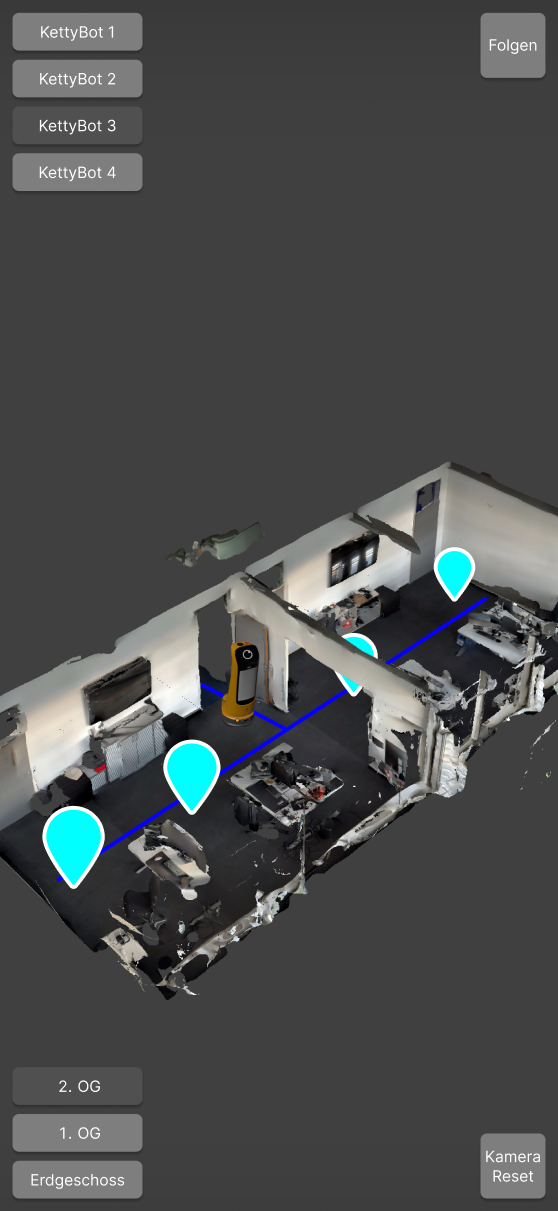
\includegraphics[width=0.65\textwidth]{Mockup Uebersicht}
\end{figure}

\begin{figure}[H]
    \centering
    \caption[]{Mockup der Steuerung}\label{fig:MockupControls}
    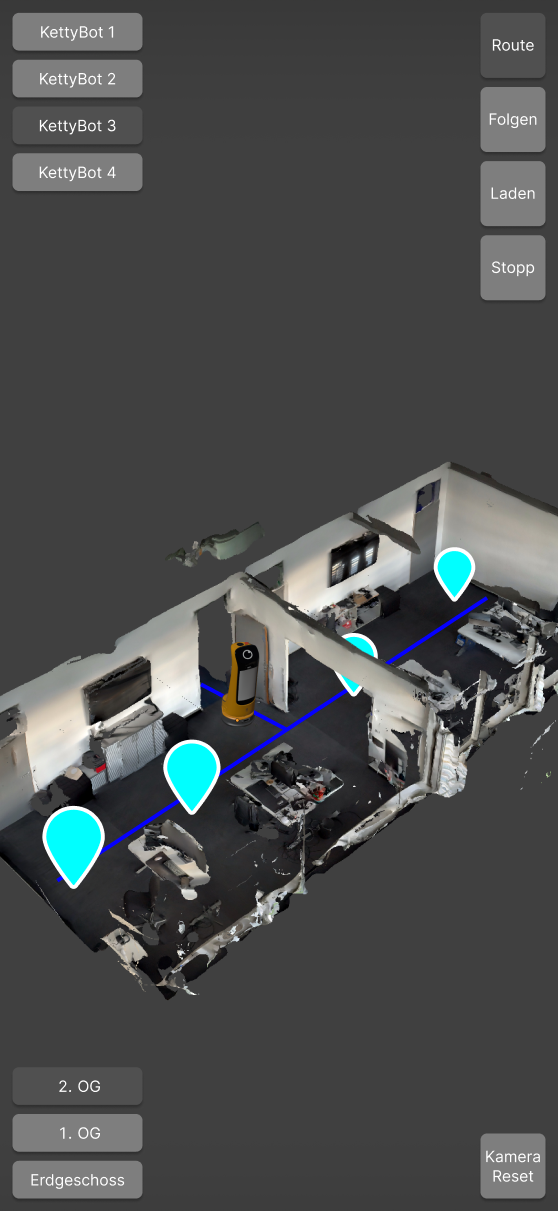
\includegraphics[width=0.65\textwidth]{Mockup Steuerung}
\end{figure}

\begin{figure}[H]
    \centering
    \caption[]{Mockup des Routenplanungs-Popup}\label{fig:MockupRoutePlanner}
    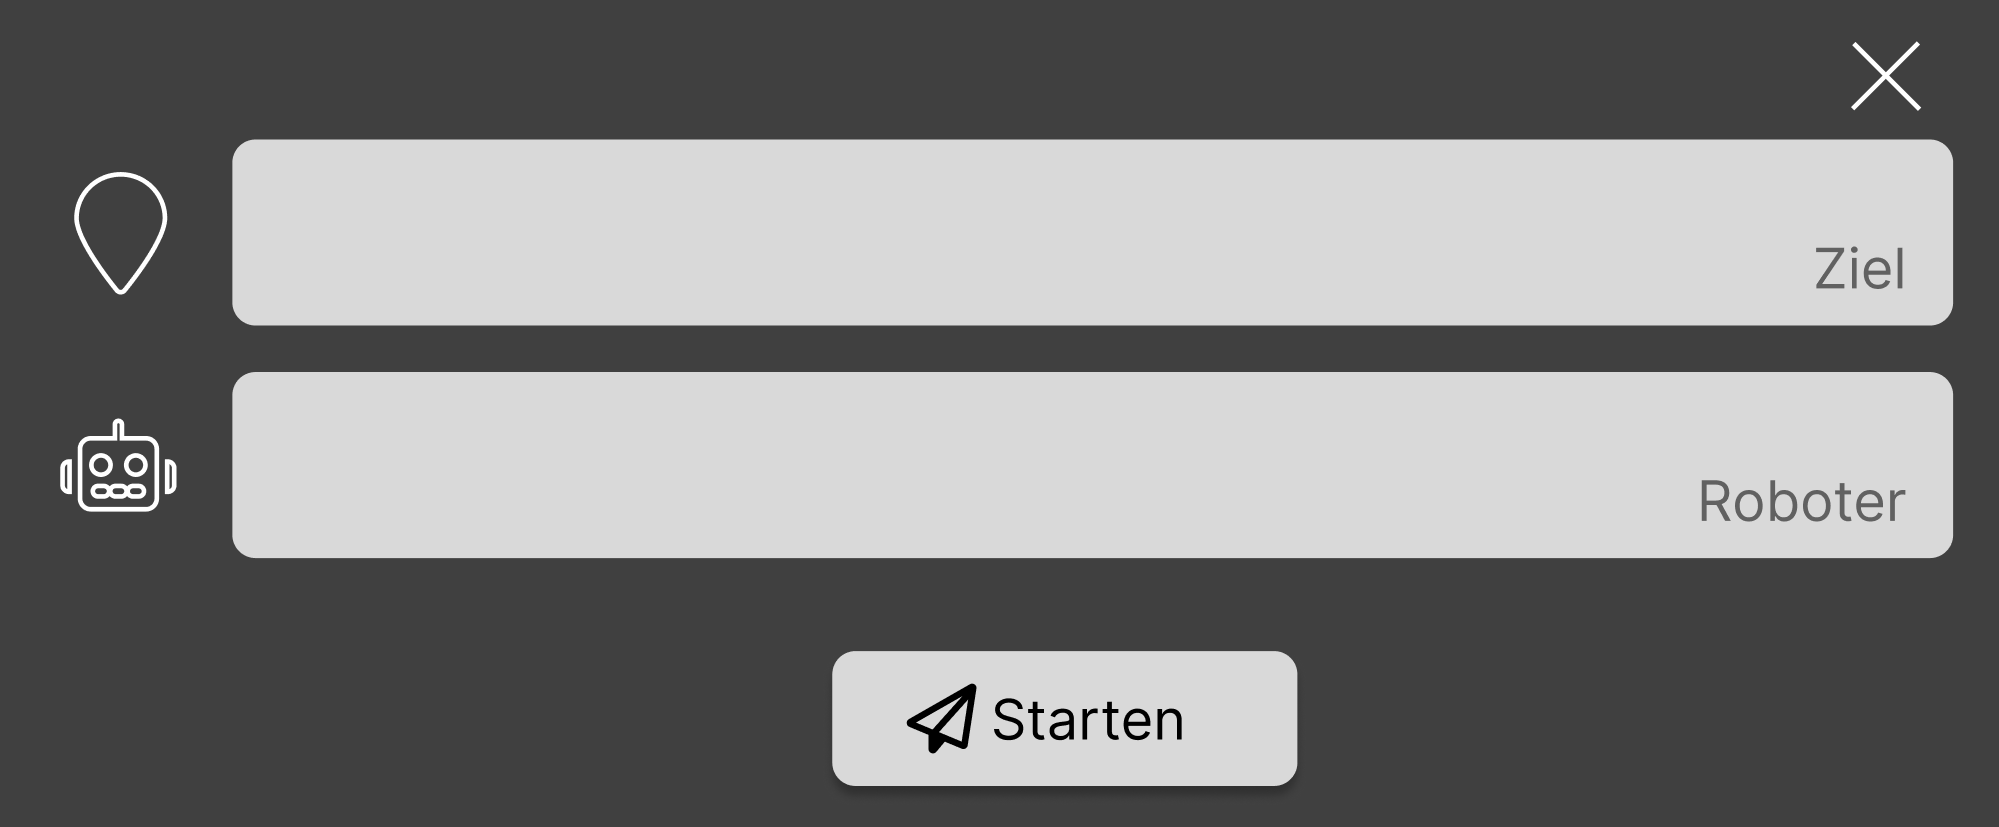
\includegraphics[width=0.65\textwidth]{Mockup Routenplaner}
\end{figure}

\begin{figure}[H]
    \centering
    \caption[]{Mockup der Verwaltung}\label{fig:MockupAdministration}
    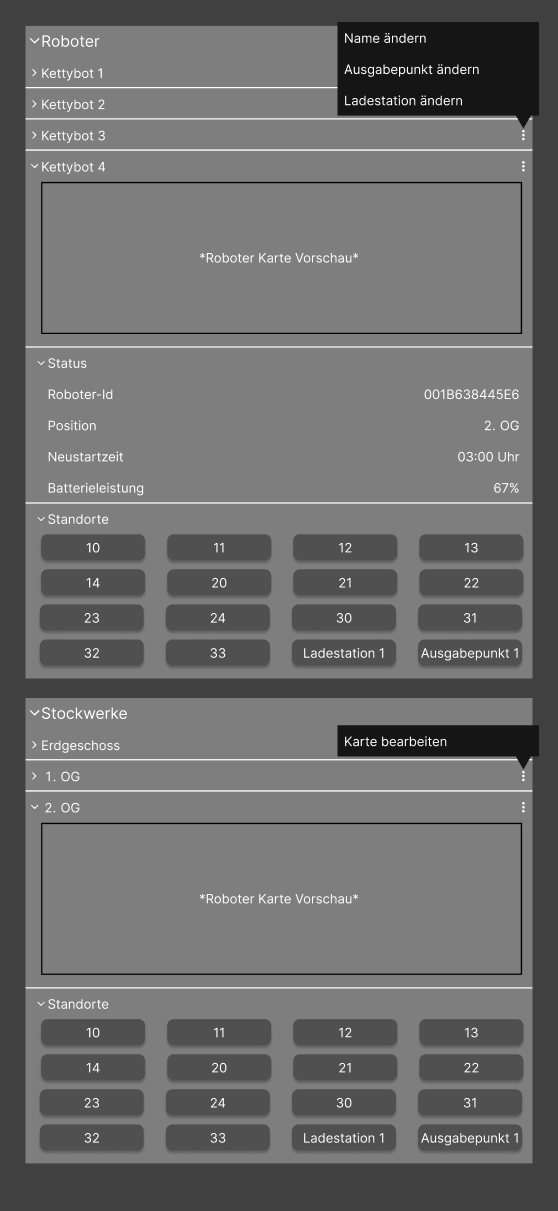
\includegraphics[width=0.65\textwidth]{Mockup Verwaltung}
\end{figure}